\documentclass{bmvc2k}
\usepackage{multicol}
\usepackage{minted}
\usepackage{float}

%% Enter your paper number here for the review copy
% \bmvcreviewcopy{??}

\title{Symulator tomografu komputerowego}

% Enter the paper's authors in order
% \addauthor{Name}{email/homepage}{INSTITUTION_CODE}
\addauthor{Maciej A. Czyzewski}{inf136698}{1}

% Enter the institutions
% \addinstitution{Name\\Address}
\addinstitution{
	Poznan University of Technology \\
	Poland
}

\runninghead{Raport}{Informatyka w Medycynie}

% Any macro definitions you would like to include
% These are not defined in the style file, because they don't begin
% with \bmva, so they might conflict with the user's own macros.
% The \bmvaOneDot macro adds a full stop unless there is one in the
% text already.
\def\eg{\emph{e.g}\bmvaOneDot}
\def\Eg{\emph{E.g}\bmvaOneDot}
\def\etal{\emph{et al}\bmvaOneDot}

%-------------------------------------------------------------------------
% Document starts here
\begin{document}

\maketitle

%-------------------------------------------------------------------------


\section{Zastosowany model tomografu}

Rownolegly (choc w projekcie zaimplementowany jest rowniez stozkowy).

\section{Zastosowany język programowania oraz dodatkowe biblioteki}

Python. Lista bibliotek (niektore sluza tylko do debugowania):

\begin{multicols}{3}
\begin{itemize}
\item watchdog==0.9.0
\item numba==0.46.0
\item tqdm==4.36.1
\item scikit\_image==0.15.0
\item numpy==1.17.2
\item pydicom==1.4.2
\item Unidecode==1.1.1
\item matplotlib==3.1.1
\item scipy==1.3.1
\item ipython==7.13.0
\item Pillow==7.0.0
\item skimage==0.0
\end{itemize}
\end{multicols}

\section{Opis głównych funkcji programu}

\subsection{pozyskiwanie odczytów dla poszczególnych detektorów}

Sinogram jest generowany funkcja {\tt fn\_tomograph} (ponizej fragment).

\begin{minted}[mathescape,
               linenos,
               numbersep=5pt,
               gobble=0,
               frame=lines,
			   framesep=2mm]{python}
# dla kolejnych detektorow
for ray in range(0, rays):
    # funkcja `d2r` zamienia stopnie na radiany
    shift = -(l / 2) + ray * l / (rays - 1)

    # tutaj mamy wsplorzedna emitera
    if not cone:  # jaki model ma byc uzyty?
        x0 = size * np.cos(d2r(i - shift))
        y0 = size * np.sin(d2r(i - shift))
    else:
        x0 = size * np.cos(d2r(i))
        y0 = size * np.sin(d2r(i))

    # po przeciwniej stronie chcemy detektor
    x1 = (size) * np.cos(d2r(i + 180 + shift))
    y1 = (size) * np.sin(d2r(i + 180 + shift))

    # tricki:
    #  - [diff_x0/diff_y0] dla przypadku
    #    gdy wejscie to prostokat
    #  - [size // 2] bo chcemy wysrodkowany
    x0 = diff_x0 + int(x0) + size // 2
    x1 = int(x1) + size // 2
    y0 = diff_y0 + int(y0) + size // 2
    y1 = int(y1) + size // 2

    # generujemy punkty na linii
    # oraz obcinamy te po za obrazkiem
    line = fn_line(x0, y0, x1, y1, X=Sw, Y=Sh)

    S = 0  # model addetywny
    for p in line:
        S += img[int(p[1]), int(p[0])]

    linogram.append(S)  # --> czyli wiersz sinogramu
    ray_lines.append([x0, y0, x1, y1])
\end{minted}

\subsection{filtrowanie sinogramu, zastosowany rozmiar maski}

Filtorwanie jak i przeksztalcenie sinogramu odbywa sie w {\tt fn\_fbp} (ponizej
fragment).

\begin{minted}[mathescape,
               linenos,
               numbersep=5pt,
               gobble=0,
               frame=lines,
			   framesep=2mm]{python}
# znaleziony filtr:
# https://www.youtube.com/watch?v=pZ7JlXagT0w
f = fftfreq(sinogram.shape[0]).reshape(-1, 1)
# f - digital frequency
omega = 2 * np.pi * f  # angular frequency
fourier_filter = 2 * np.abs(f)  # ramp filter

projection = fft(sinogram, axis=0) * fourier_filter
sinogram = np.real(ifft(projection, axis=0))
\end{minted}

Dlaczego akurat tak zrobilem, ilustruje w {\tt showcase.ipynb}.

\subsection{ustalanie jasności poszczególnych punktów obrazu wynikowego oraz
	jego przetwarzanie końcowe (np. uśrednianie, normalizacja)}

Ostatni postprocessing odbywa sie w {\tt fn\_clip}.

\begin{minted}[mathescape,
               linenos,
               numbersep=5pt,
               gobble=0,
               frame=lines,
			   framesep=2mm]{python}
def fn_clip(img, val=1.0, agressive=False):
    img = img.astype(float) * 255
    img[img < 0] = 0  # obcinamy ujemne (artefakty z ifft)
    img *= 1 / img.max() # chcemy [0, 1]

    if agressive:  # zbedny krok
        img = _fast_fn_noise_reduction(img)
        # obcinanie odchylen (najasniejszy, najciemniejszych)
        if CONFIG["rays"] >= 1000:
            p2, p98 = np.percentile(img, (0.5, 99.5))
        else:
            img = exposure.adjust_log(img, 1)
            p2, p98 = np.percentile(img, (2, 98))
        img = exposure.rescale_intensity(img, \
                                    in_range=(p2, p98))

    return img * 255
\end{minted}

\subsection{wyznaczanie wartości miary RMSE na podstawie obrazu źródłowego oraz
	wynikowego}

Wyznaczanie miary RMSE odbywa sie w {\tt fn\_calc\_rmse}.

\begin{minted}[mathescape,
               linenos,
               numbersep=5pt,
               gobble=0,
               frame=lines,
			   framesep=2mm]{python}
def fn_calc_rmse(A, B):
    A, B = fn_clip(A), fn_clip(B)
    errors = np.asarray(A - B) / 255
    return np.sqrt(np.mean(np.square(errors)))
\end{minted}

\subsection{odczyt i zapis plików DICOM}

Najlepiej sprawdzic dzialanie w pliku {\tt showcase.ipynb}.

\begin{minted}[mathescape,
               linenos,
               numbersep=5pt,
               gobble=0,
               frame=lines,
			   framesep=2mm]{python}
def do_dicom(PatientName=None, ImageComments=None, StudyDate=None):
    # edycja danych w pliku DICOM
    fn_save_dicom(
            "data/test.dcm",
            data={
                "PatientName": PatientName,
                "ImageComments": ImageComments,
                "StudyDate": StudyDate,
            },
        )

    # tutaj laduje i wyswietla dane z pliku (prefix "===")
    img = fn_load_dicom("data/test.dcm")

    # obslugujemy te pliki
    # mozna z nich robic Radon-a
    plt.figure()
    plt.imshow(img)

# interaktywne okienko / zgodnie z wymaganiami
interact_manual(do_dicom, \
        PatientName="Maciej A. Czyzewski", \
        ImageComments="Obrazek testowy, prawda?", \
        StudyDate="20200119")
\end{minted}

\section{Filtrowanie}

\begin{figure}[H]
	\begin{tabular}{ccc}
		\bmvaHangBox{\fbox{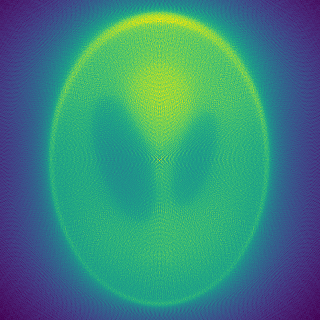
\includegraphics[width=3.6cm]{filtr_false}}} &
		\bmvaHangBox{\fbox{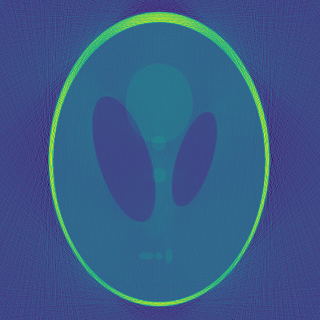
\includegraphics[width=3.6cm]{filtr_true}}} &
		\bmvaHangBox{\fbox{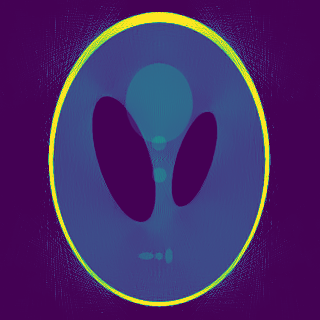
\includegraphics[width=3.6cm]{filtr_true_pre}}}\\
		(baseline)&(filtr)&(filtr+postprocessing)
\end{tabular}
\caption{Wplyw filtrowania na jakosc wizualna wyniku.}
\end{figure}

Wyraznie widac ze filtr jak i odpowieni postprocessing jest waznym elementem
procesu aby osiagnac wizualnie poprawnie obraz. Wiecej na temat zjawiska ktore
jest powodem ``rozmazania'' w {\tt showcase.ipynb}.

\begin{table}[H]
\begin{center}
\begin{tabular}{|l|c|}
\hline
Method & RMSE \\
\hline\hline
baseline & 0.5087 \\
filtr & 0.1142 \\
filtr+postprocessing & \textbf{0.0916} \\
\hline
\end{tabular}
\end{center}
\caption{Wplyw filtrowania na RMSE.}
\end{table}

\section{Wynik eksperymentu}

Tak. Wnioski wynikające z przebiegow są zgodne z oceną subiektywną jakości obrazu.

\begin{figure}[H]
	\begin{tabular}{cc}
		\bmvaHangBox{\fbox{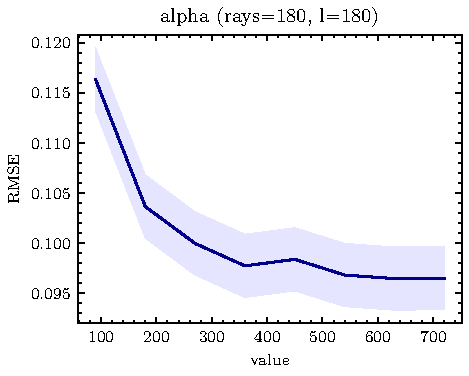
\includegraphics[width=5.8cm]{figure-1-alpha-rays-180-l-180}}}&
		\bmvaHangBox{\fbox{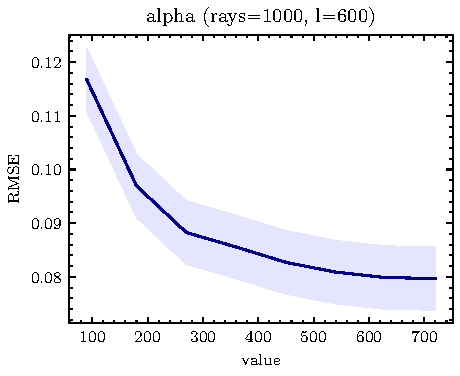
\includegraphics[width=5.8cm]{figure-2-alpha-rays-1000-l-600}}}\\
(a)&(b)
\end{tabular}
\caption{Wplyw kroku $\Delta\alpha$ układu emiter/detektor na RMSE.} 
\end{figure}


\begin{figure}[H]
	\begin{tabular}{cc}
		\bmvaHangBox{\fbox{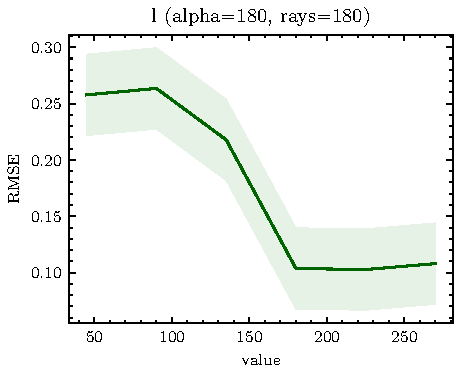
\includegraphics[width=5.8cm]{figure-1-l-alpha-180-rays-180}}}&
		\bmvaHangBox{\fbox{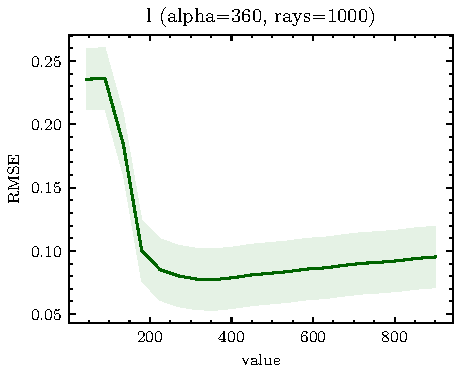
\includegraphics[width=5.8cm]{figure-2-l-alpha-360-rays-1000}}}\\
(a)&(b)
\end{tabular}
\caption{Wplyw rozwartości/rozpiętości układu emiter/detektor na RMSE.}
\end{figure}


\begin{figure}[H]
	\begin{tabular}{cc}
		\bmvaHangBox{\fbox{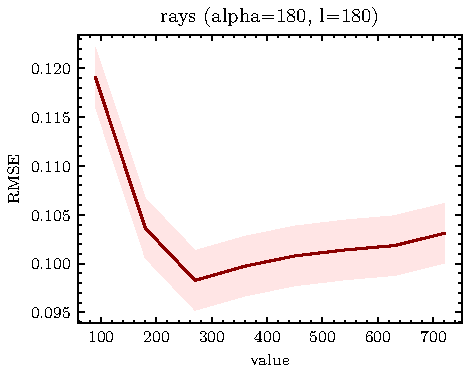
\includegraphics[width=5.8cm]{figure-1-rays-alpha-180-l-180}}}&
		\bmvaHangBox{\fbox{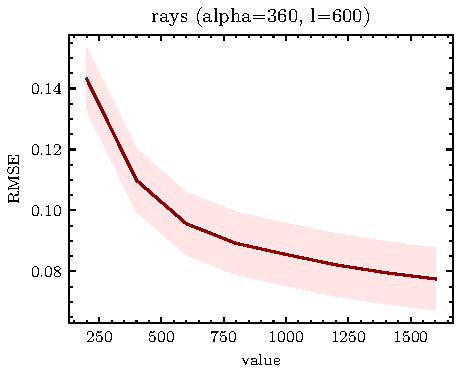
\includegraphics[width=5.8cm]{figure-2-rays-alpha-360-l-600}}}\\
(a)&(b)
\end{tabular}
\caption{Wplyw liczby detektorów układu emiter/detektor na RMSE.}
\end{figure}

Przebiegi dla eksperymentu z wartosciami poczatkowymi ustawionymi na 180 na
kazdym parametrze byly niesatyskacjunujace (a); dlatego zostaly dla porownania
wygenerowane dla duzo wiekszy wartosci/rozdzielczosci (b).

Zgodnie z oczekiwaniami zwiekszenie liczby detektorow zwieksza jakosc obrazu
(wymiar Y sinogramu sie zwieksza) wiec mamy zakodowane wieksza ilosc informacji.
Podobnie jest z parametrem $\alpha$ ktory natomiast powoduje ze mamy coraz
wieksza gestosc pomiarow w wymiarze X (czyli na polowe pelnego obrotu).
Parametr rozpietosci; $l$ jest troche trudniejszy do interpretacji, nie
powinnien on monotonicznie wplywac na RMSE, gdy zsumujemy wartosci promienii dla
pustego obrazka zobaczymy ``pregi''. Najlepiej wybrac takie $l$ ktore dla danych
pozostalych parametrow stworzy jak najmniej takich nieporzadanych kolek.
Dodatkowo zbyt male $l$ nie bedzie zbierac informacji z calego obrazka, zbyt
duze zacznie oslabiac nam znaczenie detektorow zewnetrznych.

\end{document}
